\renewcommand{\newCommandChapterTitle}{Pruebas y resultados}
\chapter{\newCommandChapterTitle}
\markright{\hfill \thechapter. \newCommandChapterTitle}
\label{chap:p3_results}


En este capítulo presentamos las pruebas que realizamos con \gls{acr3:name}.
Primeramente describimos los conjuntos de datos de prueba utilizados,
luego explicamos las pruebas realizadas y finalmente comparamos los
resultados obtenidos con otros trabajos relacionados.


\section{Conjuntos de datos de prueba}

Para evaluaciones cuantitativas de la eficacia de detección del
\gls{acr3:waf} que hemos implementado necesitamos conjuntos de datos.
Obtener buenos datos para las pruebas es fundamental para obtener
resultados que después se comprueben en el mundo real.
Pero esto no es una tarea fácil, ya que muchos conjuntos de datos tienen
ciertas falencias que los hacen poco útiles para nuestras pruebas
\citep{torranoGimenez2015study}.

\subsection{Características deseadas para los conjuntos de datos}

Según \citep{torranoGimenez2015study} los conjuntos de
datos utilizados en las investigaciones sobre \gls{acr3:waf} deberían
cumplir ciertos criterios para ser de utilidad para la comunidad
científica. Algunas de esas características son:

\begin{itemize}
    \item
    Deberían ser públicos para que investigadores puedan comparar
    resultados.

    \item
    Deberían contener tráfico \gls{acr3:http}, ya que se trata de un
    \gls{acr3:waf}.

    \item
    Deberían contener datos etiquetados según sean normales o anómalas.

    \item
    Deberían incluir ataques novedosos y relevantes.
\end{itemize}

Los trabajos relacionados sobre \gls{acr3:waf} utilizan distintos conjuntos
de datos para sus pruebas, pero la mayoría de esos conjuntos no cumple una
o varias de las características mencionadas anteriormente
\citep{torranoGimenez2015study}.
Encontramos dos conjuntos de datos adecuados según los criterios mencionados;
fueron creados por el Consejo Superior de Investigaciones Científicas
(\gls{acr3:csic}) de España y publicados como \gls{acr3:csic} 2010
\citep{csic2010dataset} y \gls{acr3:csic} TORPEDA 2012 \citep{torpeda2012dataset}.
Varias investigaciones relacionadas ya utilizaron estos conjuntos, como
por ejemplo \citep{parhizkar2015oc} y \citep{torranoGimenez2015study},
y así podemos comparar resultados con dichos trabajos.


\subsection{Descripción de los conjuntos de datos utilizados}

Los dos conjuntos de datos del \gls{acr3:csic} contienen peticiones
\gls{acr3:http} hechas a una aplicación sencilla de comercio electrónico,
simulando distintos escenarios como, por ejemplo, registro de clientes
y compra de productos. Una descripción más detallada sobre el proceso
de creación de estos conjuntos se puede encontrar en el trabajo
\citep{torranoGimenez2015study}.

El conjunto \gls{acr3:csic} 2010 \citep{csic2010dataset} consiste de tres
archivos: dos archivos de 20 \gls{acr3:mb} con tráfico \gls{acr3:http}
normal, que contienen alrededor de \num{72000} peticiones, y un archivo
de 15 \gls{acr3:mb} con tráfico anómalo, que contiene cerca de \num{25000}
peticiones. Este último archivo contiene varios tipos de ataques, además
de anomalías que no necesariamente son ataques pero representan peticiones
con datos no esperados.

Considerando que nuestro \gls{acr3:waf} entrena un clasificador por cada
combinación de \gls{acr3:url} y método \gls{acr3:http}, nosotros agrupamos
todas las peticiones de los tres archivos por este criterio.
De esta manera obtuvimos más de \num{1600} grupos distintos, pero notamos
que muchos de ellos tenían solamente peticiones normales o solamente
peticiones anómalas. Esos casos no nos sirven para las pruebas, ya que
necesitamos datos normales para el entrenamiento y posteriormente anomalías
para validar que el \gls{acr3:waf} detecta correctamente estas últimas.
Por este motivo decidimos utilizar solamente aquellos grupos que tienen
más de 100 peticiones normales y también más de 100 peticiones anómalas.
Así obtuvimos 16 grupos, alcanzando un total de \num{32000} peticiones
normales y \num{19160} anómalas.
En la \autoref{tbl:res:selected_data_sets} se pueden ver en detalle los grupos
de peticiones que utilizamos para nuestras pruebas, incluyendo un identificador
corto que le asignamos a cada uno de los grupos para la mejor visualización
de los resultados.

El conjunto de datos \gls{acr3:csic} TORPEDA 2012 \citep{torpeda2012dataset}
consiste de ocho archivos: un archivo de 8 \gls{acr3:mb} con tráfico
\gls{acr3:http} normal, que contiene alrededor de \num{8000} peticiones,
y siete archivos totalizando más de 60 \gls{acr3:mb} de tráfico anómalo,
que contienen más de \num{65000} peticiones con ataques y también anomalías
no maliciosas.

\begin{table}[ht]
    \centering
    \small
    \begin{tabularx}{\linewidth}{|C|c|ll|r|r|r|}
        \hline
        ID
        & \multicolumn{1}{c|}{\begin{tabular}[c]{@{}c@{}}Conjunto\\ de datos\\ CSIC\end{tabular}}
        & \multicolumn{2}{c|}{Método HTTP y URL}
        & \multicolumn{1}{c|}{\begin{tabular}[c]{@{}c@{}}Cant.\\ parám.\end{tabular}}
        & \multicolumn{1}{c|}{\begin{tabular}[c]{@{}c@{}}Peticiones\\ normales\end{tabular}}
        & \multicolumn{1}{c|}{\begin{tabular}[c]{@{}c@{}}Peticiones\\ anómalas\end{tabular}} \\
        \specialrule{1.5pt}{0}{0}
        c00 & 2010  & GET  & /tienda1/miembros/editar.jsp         & 13 &  \num{2000} &  \num{1362} \\ \hline
        c01 & 2010  & POST & /tienda1/miembros/editar.jsp         & 13 &  \num{2000} &  \num{1362} \\ \hline
        c02 & 2010  & GET  & /tienda1/publico/anadir.jsp          &  5 &  \num{2000} &  \num{1380} \\ \hline
        c03 & 2010  & POST & /tienda1/publico/anadir.jsp          &  5 &  \num{2000} &  \num{1380} \\ \hline
        c04 & 2010  & GET  & /tienda1/publico/autenticar.jsp      &  5 &  \num{2000} &  \num{1361} \\ \hline
        c05 & 2010  & POST & /tienda1/publico/autenticar.jsp      &  5 &  \num{2000} &  \num{1361} \\ \hline
        c06 & 2010  & GET  & /tienda1/publico/caracteristicas.jsp &  1 &  \num{2000} &   \num{954} \\ \hline
        c07 & 2010  & POST & /tienda1/publico/caracteristicas.jsp &  1 &  \num{2000} &   \num{954} \\ \hline
        c08 & 2010  & GET  & /tienda1/publico/entrar.jsp          &  1 &  \num{2000} &   \num{897} \\ \hline
        c09 & 2010  & POST & /tienda1/publico/entrar.jsp          &  1 &  \num{2000} &   \num{897} \\ \hline
        c10 & 2010  & GET  & /tienda1/publico/pagar.jsp           &  3 &  \num{2000} &  \num{1343} \\ \hline
        c11 & 2010  & POST & /tienda1/publico/pagar.jsp           &  3 &  \num{2000} &  \num{1343} \\ \hline
        c12 & 2010  & GET  & /tienda1/publico/registro.jsp        & 13 &  \num{2000} &  \num{1364} \\ \hline
        c13 & 2010  & POST & /tienda1/publico/registro.jsp        & 13 &  \num{2000} &  \num{1364} \\ \hline
        c14 & 2010  & GET  & /tienda1/publico/vaciar.jsp          &  1 &  \num{2000} &   \num{919} \\ \hline
        c15 & 2010  & POST & /tienda1/publico/vaciar.jsp          &  1 &  \num{2000} &   \num{919} \\ \hline
        t00 & 2012  & POST & /tienda1/miembros/editar.jsp         & 12 &  \num{5608} & \num{10121} \\ \hline
        t01 & 2012  & POST & /tienda1/publico/registro.jsp        & 12 &  \num{2522} & \num{13163} \\
        \specialrule{1.5pt}{0}{0}
            & Total &      &                                      &    & \num{40130} & \num{42444} \\ \hline
    \end{tabularx}

    \caption{Peticiones seleccionadas de los conjuntos de datos para nuestras
        pruebas, agrupadas por método \gls{acr3:http} y \gls{acr3:url}.}
    \label{tbl:res:selected_data_sets}
\end{table}

Realizando de vuelta la agrupación de las peticiones obtuvimos 72 grupos
distintos, pero también había casos con solamente peticiones normales
o solamente anomalías. Después de seleccionar únicamente aquellos con
más de 100 peticiones normales y también más de 100 peticiones anómalas,
nos quedamos con 2 grupos, alcanzando un total de \num{8130} peticiones
normales y \num{23284} anómalas.
En la ya mencionada \autoref{tbl:res:selected_data_sets} se pueden ver los
detalles de estos grupos también.


\section{Análisis de la eficacia de detección}

Realizamos pruebas para analizar la eficacia de detección de \gls{acr3:name},
utilizando los conjuntos de datos presentados. Con el fin de agilizar el
proceso de extracción de \textit{features} y realizar la clasificación
de forma más eficiente, para estas pruebas construimos una versión
reducida del \gls{acr3:waf} que no incluye recepción y envío de peticiones,
sino que obtiene las peticiones de un archivo. El código se encuentra en
el directorio \path{/tests/detection_efficacy/}.

Cabe volver a mencionar que nuestra implementación no contiene todavía
un mecanismo automático para la selección de los valores para los parámetros
\gls{sim3:nui} y \gls{sim3:gammai} de los clasificadores. Para estas
pruebas, realizamos una búsqueda en el rango $[\num{0.0001} ; \num{0.1}]$
para ambos parámetros y seleccionamos los valores que obtuvieron los
mejores resultados en la fase de detección para cada grupo de peticiones.
Cada búsqueda fue realizada tres veces, utilizando cada vez un subconjunto
distinto de peticiones para el entrenamiento, con el fin de evitar resultados
dependientes de la selección particular de muestras.
Con esto metodología utilizada mostramos que existen valores para los
parámetros \gls{sim3:nui} y \gls{sim3:gammai} de los clasificadores con
los cuales se puede obtener los resultados de detección que son presentados
a continuación.

\begin{figure}[th]
    \centering
    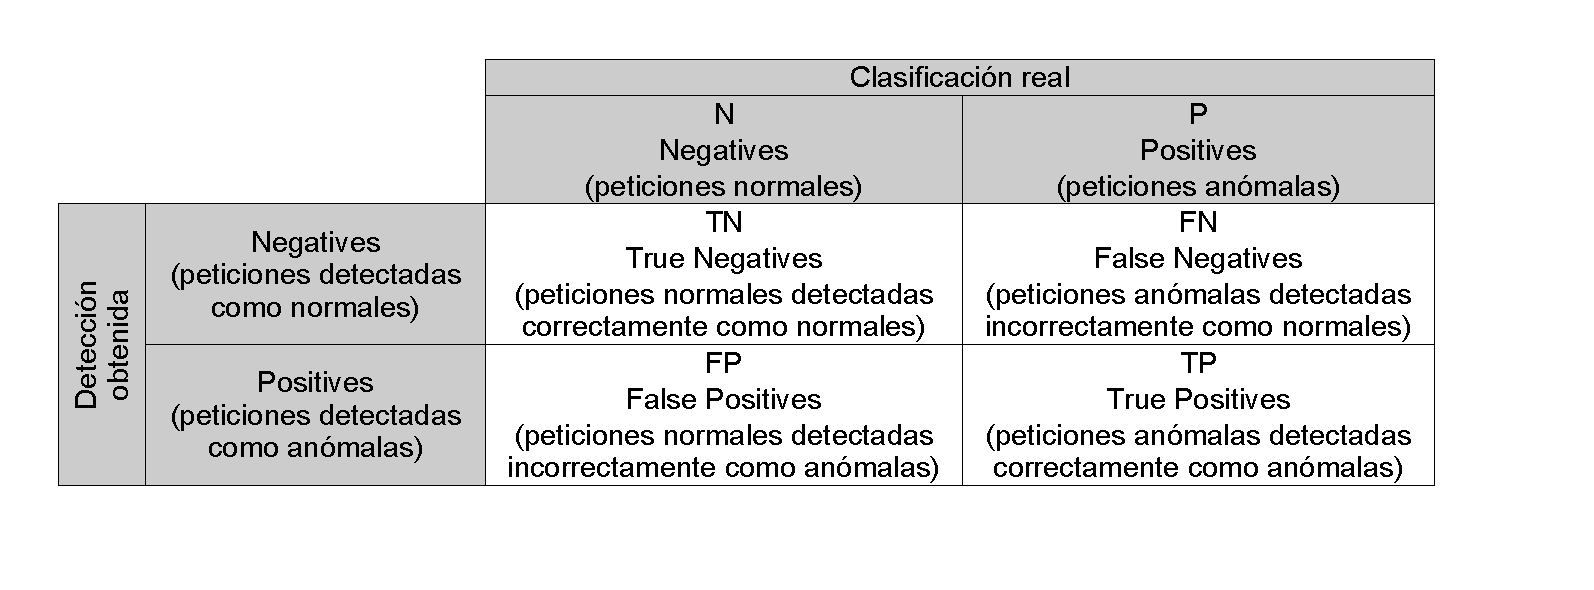
\includegraphics[width=\linewidth, trim=1.1cm 1.7cm 1.6cm 1cm]{images/diagram-score-explanation.pdf}

    \caption{Matriz de confusión de los posibles resultados de clasificación.}
    \label{fig:res:score_explanation}
\end{figure}

Para la cuantificación de las pruebas, tomamos en cuenta los distintos
resultados de clasificación que se puede obtener en la terminología de
\gls{acr3:ids}, según la matriz de confusión ilustrada en la
\autoref{fig:res:score_explanation}.
Se puede observar que la cantidad total de peticiones en la fase de
detección se compone de las peticiones normales (N, o muestras negativas)
y las anomalías o ataques (P, o muestras positivas).

Las peticiones normales pueden ser detectadas como tales, resultando en
negativos correctos (TN), o pueden ser detectadas como peticiones no
pertenecientes a la clase conocida de los normales, resultando en falsos
positivos (FP).
De la misma forma, las peticiones anómalas pueden ser detectadas como
tales, resultando en positivos correctos (TP), o pueden ser detectadas
erróneamente como pertenecientes a los mensajes normales, resultando en
falsos negativos (FN).
Estas cantidades y las relaciones entre ellas también pueden ser expresadas
como se puede observar en la \autoref{eq:res:scores1}.

\begin{equation}
    \label{eq:res:scores1}
    \text{Total de muestras} = \text{N} + \text{P}
    \ , \quad
    \text{N} = \text{TN} + \text{FP}
    \ , \quad
    \text{P} = \text{TP} + \text{FN}
\end{equation}

Para el análisis de nuestros resultados utilizamos varias métricas que
son fórmulas agregadas de estas cantidades vistas.

\begin{itemize}
    \item
    \textit{True Positives Rate} (\gls{acr3:tpr}):
    Esta métrica indica la fracción de peticiones anómalas (muestras
    positivas) que fue detectada correctamente; tiene un rango $[0;1]$.
    El valor debería ser cercano a 1 para que el \gls{acr3:waf} detecte
    la mayor cantidad posible de ataques antes de que lleguen a las
    aplicaciones protegidas.

    \item
    \textit{False Positives Rate} (\gls{acr3:fpr}):
    Esta métrica indica la fracción de peticiones normales (muestras
    negativas) que fue detectada equivocadamente como anomalías; tiene
    un rango $[0;1]$.
    El valor debería ser cercano a 0 para que el \gls{acr3:waf} no afecte
    negativamente la experiencia de usuarios legítimos de las aplicaciones
    protegidas al bloquear peticiones normales.

    \item
    F$_{1}$-\textit{score}:
    Esta métrica busca incorporar las dos métricas anteriores en un solo
    indicador; tiene también un rango $[0;1]$.
    El valor debería ser también cercano a 1 en los resultados producidos
    por el \gls{acr3:waf} para cumplir los dos objetivos mencionados
    acerca del \gls{acr3:tpr} (detectar todos los ataques) y \gls{acr3:fpr}
    (no afectar usuarios legítimos).
\end{itemize}

Estas tres métricas pueden ser expresadas también con las expresiones
que podemos observar en la \autoref{eq:res:scores2}.

\begin{equation}
    \label{eq:res:scores2}
    \text{TPR} = \frac{\text{TP}}{\text{P}}
    \ , \quad
    \text{FPR} = \frac{\text{FP}}{\text{N}}
    \ , \quad
    \text{F}_{1} = \frac{2 \text{TP}}{2 \text{TP} + \text{FP} + \text{FN}}
\end{equation}

En el análisis de la eficacia de detección de \gls{acr3:name} nos enfocamos
en cuatro aspectos; las mejoras obtenidas por incluir el escalamiento de
los \textit{features}, las mejoras que produce el análisis de los valores
de los parámetros en las peticiones, la influencia de la cantidad de
peticiones utilizadas para el entrenamiento y finalmente la influencia
de peticiones anómalas presentes en los datos de entrenamiento.


\subsection{Mejoras obtenidas por el escalamiento de \textit{features}}

Como ya explicamos en el \autoref{chap:p3_concepts_features}, después
de la extracción de \textit{features} realizamos un escalamiento para
obtener promedio cercano a 0 y varianza cercana a 1 para cada \textit{feature}
de los datos de entrenamiento. Según la teoría, este preprocesamiento ayuda
a mejorar la capacidad de clasificación del \gls{acr3:ocsvm}
\citep{rieck2009machine}, % from section 2.3.1 - normalization of numerical features
y con los resultados de esta prueba logramos comprobar esto.

\begin{table}[ht]
    \centering
    \small
    \begin{tabularx}{\linewidth}{|c|CCC|CCC|}
        \hline
        ID  & \multicolumn{3}{c|}{Sin escalamiento}                                                   & \multicolumn{3}{c|}{Con escalamiento}                                                   \\
            & \gls{acr3:tpr}              & \gls{acr3:fpr}              & F$_{1}$-\textit{score}      & \gls{acr3:tpr}              & \gls{acr3:fpr}              & F$_{1}$-\textit{score}      \\
        \specialrule{1.5pt}{0}{0}
        c00 & \num{0.85} $\pm$ \num{0.01} & \num{0.31} $\pm$ \num{0.01} & \num{0.73} $\pm$ \num{0.00} & \num{0.71} $\pm$ \num{0.01} & \num{0.05} $\pm$ \num{0.00} & \num{0.80} $\pm$ \num{0.00} \\ \hline
        c01 & \num{0.85} $\pm$ \num{0.00} & \num{0.32} $\pm$ \num{0.00} & \num{0.73} $\pm$ \num{0.00} & \num{0.72} $\pm$ \num{0.01} & \num{0.05} $\pm$ \num{0.01} & \num{0.80} $\pm$ \num{0.00} \\ \hline
        c02 & \num{0.93} $\pm$ \num{0.12} & \num{0.13} $\pm$ \num{0.10} & \num{0.88} $\pm$ \num{0.01} & \num{1.00} $\pm$ \num{0.00} & \num{0.03} $\pm$ \num{0.01} & \num{0.98} $\pm$ \num{0.01} \\ \hline
        c03 & \num{0.87} $\pm$ \num{0.12} & \num{0.08} $\pm$ \num{0.12} & \num{0.88} $\pm$ \num{0.01} & \num{1.00} $\pm$ \num{0.00} & \num{0.03} $\pm$ \num{0.00} & \num{0.98} $\pm$ \num{0.00} \\ \hline
        c04 & \num{0.97} $\pm$ \num{0.01} & \num{0.25} $\pm$ \num{0.01} & \num{0.83} $\pm$ \num{0.01} & \num{0.91} $\pm$ \num{0.01} & \num{0.01} $\pm$ \num{0.00} & \num{0.95} $\pm$ \num{0.01} \\ \hline
        c05 & \num{0.96} $\pm$ \num{0.01} & \num{0.26} $\pm$ \num{0.01} & \num{0.82} $\pm$ \num{0.01} & \num{0.92} $\pm$ \num{0.01} & \num{0.01} $\pm$ \num{0.00} & \num{0.95} $\pm$ \num{0.00} \\ \hline
        c06 & \num{0.99} $\pm$ \num{0.00} & \num{0.08} $\pm$ \num{0.06} & \num{0.92} $\pm$ \num{0.05} & \num{0.99} $\pm$ \num{0.00} & \num{0.00} $\pm$ \num{0.00} & \num{1.00} $\pm$ \num{0.00} \\ \hline
        c07 & \num{0.99} $\pm$ \num{0.01} & \num{0.11} $\pm$ \num{0.01} & \num{0.88} $\pm$ \num{0.01} & \num{0.99} $\pm$ \num{0.00} & \num{0.00} $\pm$ \num{0.00} & \num{1.00} $\pm$ \num{0.00} \\ \hline
        c08 & \num{0.99} $\pm$ \num{0.02} & \num{0.01} $\pm$ \num{0.00} & \num{0.98} $\pm$ \num{0.01} & \num{1.00} $\pm$ \num{0.00} & \num{0.00} $\pm$ \num{0.00} & \num{1.00} $\pm$ \num{0.00} \\ \hline
        c09 & \num{0.98} $\pm$ \num{0.03} & \num{0.01} $\pm$ \num{0.01} & \num{0.99} $\pm$ \num{0.02} & \num{1.00} $\pm$ \num{0.00} & \num{0.00} $\pm$ \num{0.00} & \num{1.00} $\pm$ \num{0.00} \\ \hline
        c10 & \num{1.00} $\pm$ \num{0.00} & \num{0.14} $\pm$ \num{0.03} & \num{0.90} $\pm$ \num{0.02} & \num{1.00} $\pm$ \num{0.00} & \num{0.00} $\pm$ \num{0.00} & \num{1.00} $\pm$ \num{0.00} \\ \hline
        c11 & \num{1.00} $\pm$ \num{0.00} & \num{0.16} $\pm$ \num{0.02} & \num{0.90} $\pm$ \num{0.01} & \num{1.00} $\pm$ \num{0.00} & \num{0.01} $\pm$ \num{0.00} & \num{0.99} $\pm$ \num{0.00} \\ \hline
        c12 & \num{0.86} $\pm$ \num{0.01} & \num{0.31} $\pm$ \num{0.02} & \num{0.75} $\pm$ \num{0.01} & \num{0.74} $\pm$ \num{0.00} & \num{0.05} $\pm$ \num{0.01} & \num{0.81} $\pm$ \num{0.01} \\ \hline
        c13 & \num{0.86} $\pm$ \num{0.01} & \num{0.32} $\pm$ \num{0.01} & \num{0.74} $\pm$ \num{0.00} & \num{0.74} $\pm$ \num{0.00} & \num{0.05} $\pm$ \num{0.01} & \num{0.81} $\pm$ \num{0.01} \\ \hline
        c14 & \num{0.96} $\pm$ \num{0.04} & \num{0.01} $\pm$ \num{0.01} & \num{0.97} $\pm$ \num{0.02} & \num{1.00} $\pm$ \num{0.00} & \num{0.00} $\pm$ \num{0.00} & \num{1.00} $\pm$ \num{0.00} \\ \hline
        c15 & \num{0.94} $\pm$ \num{0.01} & \num{0.01} $\pm$ \num{0.01} & \num{0.96} $\pm$ \num{0.00} & \num{1.00} $\pm$ \num{0.00} & \num{0.00} $\pm$ \num{0.00} & \num{1.00} $\pm$ \num{0.00} \\ \hline
        t00 & \num{1.00} $\pm$ \num{0.00} & \num{0.07} $\pm$ \num{0.04} & \num{0.98} $\pm$ \num{0.01} & \num{0.99} $\pm$ \num{0.01} & \num{0.06} $\pm$ \num{0.04} & \num{0.98} $\pm$ \num{0.00} \\ \hline
        t01 & \num{0.99} $\pm$ \num{0.01} & \num{0.09} $\pm$ \num{0.10} & \num{0.99} $\pm$ \num{0.01} & \num{1.00} $\pm$ \num{0.00} & \num{0.09} $\pm$ \num{0.06} & \num{0.99} $\pm$ \num{0.01} \\
        \specialrule{1.5pt}{0}{0}
            & \num{0.94} $\pm$ \num{0.07} & \num{0.15} $\pm$ \num{0.12} & \num{0.88} $\pm$ \num{0.09} & \num{0.93} $\pm$ \num{0.11} & \num{0.03} $\pm$ \num{0.03} & \num{0.95} $\pm$ \num{0.08} \\ \hline
    \end{tabularx}

    \caption{Resultados de detección que muestran las mejoras obtenidas
        por el escalamiento de \textit{features}, incluyendo el análisis
        de valores de parámetros.}
    \label{tbl:res:results_scaling}
\end{table}

En la \autoref{tbl:res:results_scaling} se puede observar los resultados
de la clasificación sin y con escalamiento. Para ambos casos usamos 1500
peticiones para el entrenamiento de cada grupo (cerca del 75\% de las
muestras) e incluimos los \textit{features} del análisis de valores de
parámetros.
Al observar los resultados promedios de los grupos de peticiones (la
última fila de la tabla), se puede ver que con el escalamiento el
F$_{1}$-\textit{score} aumenta de \num{0.88} y \num{0.95}, ya que a
pesar de que el \gls{acr3:tpr} promedio baja de \num{0.94} a \num{0.93},
el \gls{acr3:fpr} mejora considerablemente de \num{0.15} a \num{0.03}.

Estos resultados pueden ser observados también en forma gráfica en la
\autoref{fig:res:results_scaling}, donde se compara el F$_{1}$-\textit{score}
obtenido en el proceso de detección sin y con escalamiento para cada
uno de los 18 grupos de peticiones.

\begin{figure}[ht]
    \centering
    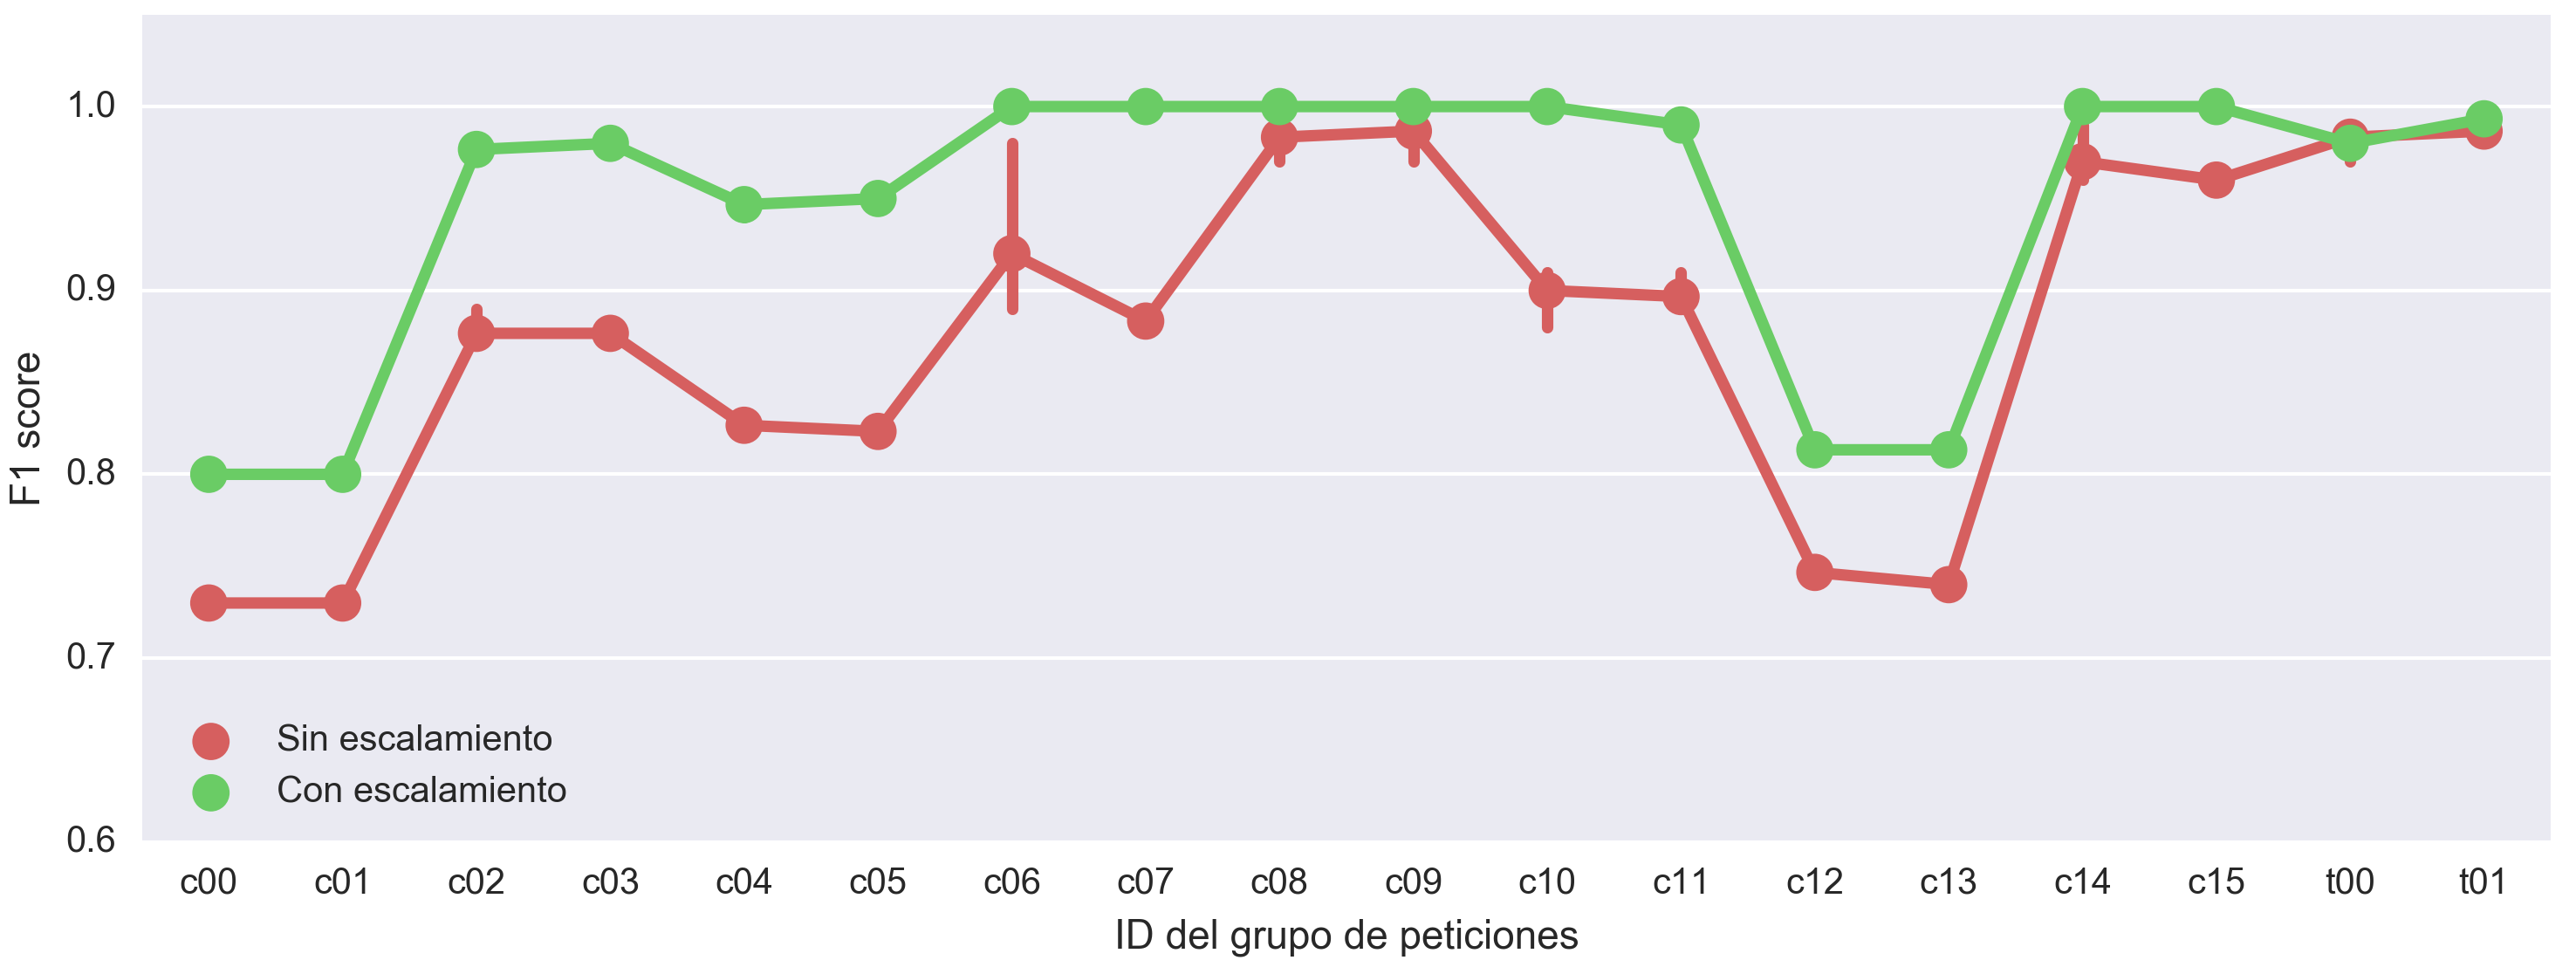
\includegraphics[width=\linewidth]{images/results-scaling.png}

    \caption{Resultados de detección que muestran las mejoras obtenidas
        por el escalamiento de \textit{features}, incluyendo el análisis
        de valores de parámetros.}
    \label{fig:res:results_scaling}
\end{figure}

De esta forma, los resultados nos confirman que el escalamiento de los
\textit{features} mejora la capacidad de clasificación de nuestro
\gls{acr3:ocsvm} para la detección de anomalías en peticiones \gls{acr3:http},
al menos para el conjunto de datos que utilizamos.


\subsection{Mejoras obtenidas por el análisis de valores de parámetros}

Nuestros procesos de extracción de \textit{features} en primer lugar
analizan la petición completa, que resulta en una cantidad fija de
\textit{features} que se obtiene para cada petición.
Adicionalmente, estos procesos analizan también los valores de los
parámetros del \textit{query string} y del cuerpo de las peticiones,
lo que resulta en \textit{features} adicionales cuya cantidad depende
de la cantidad de parámetros de las peticiones de cada grupo. En esta
prueba mostramos que estos \textit{features} adicionales pueden mejorar
la detección de \gls{acr3:name}.

\begin{figure}[hbt]
    \centering
    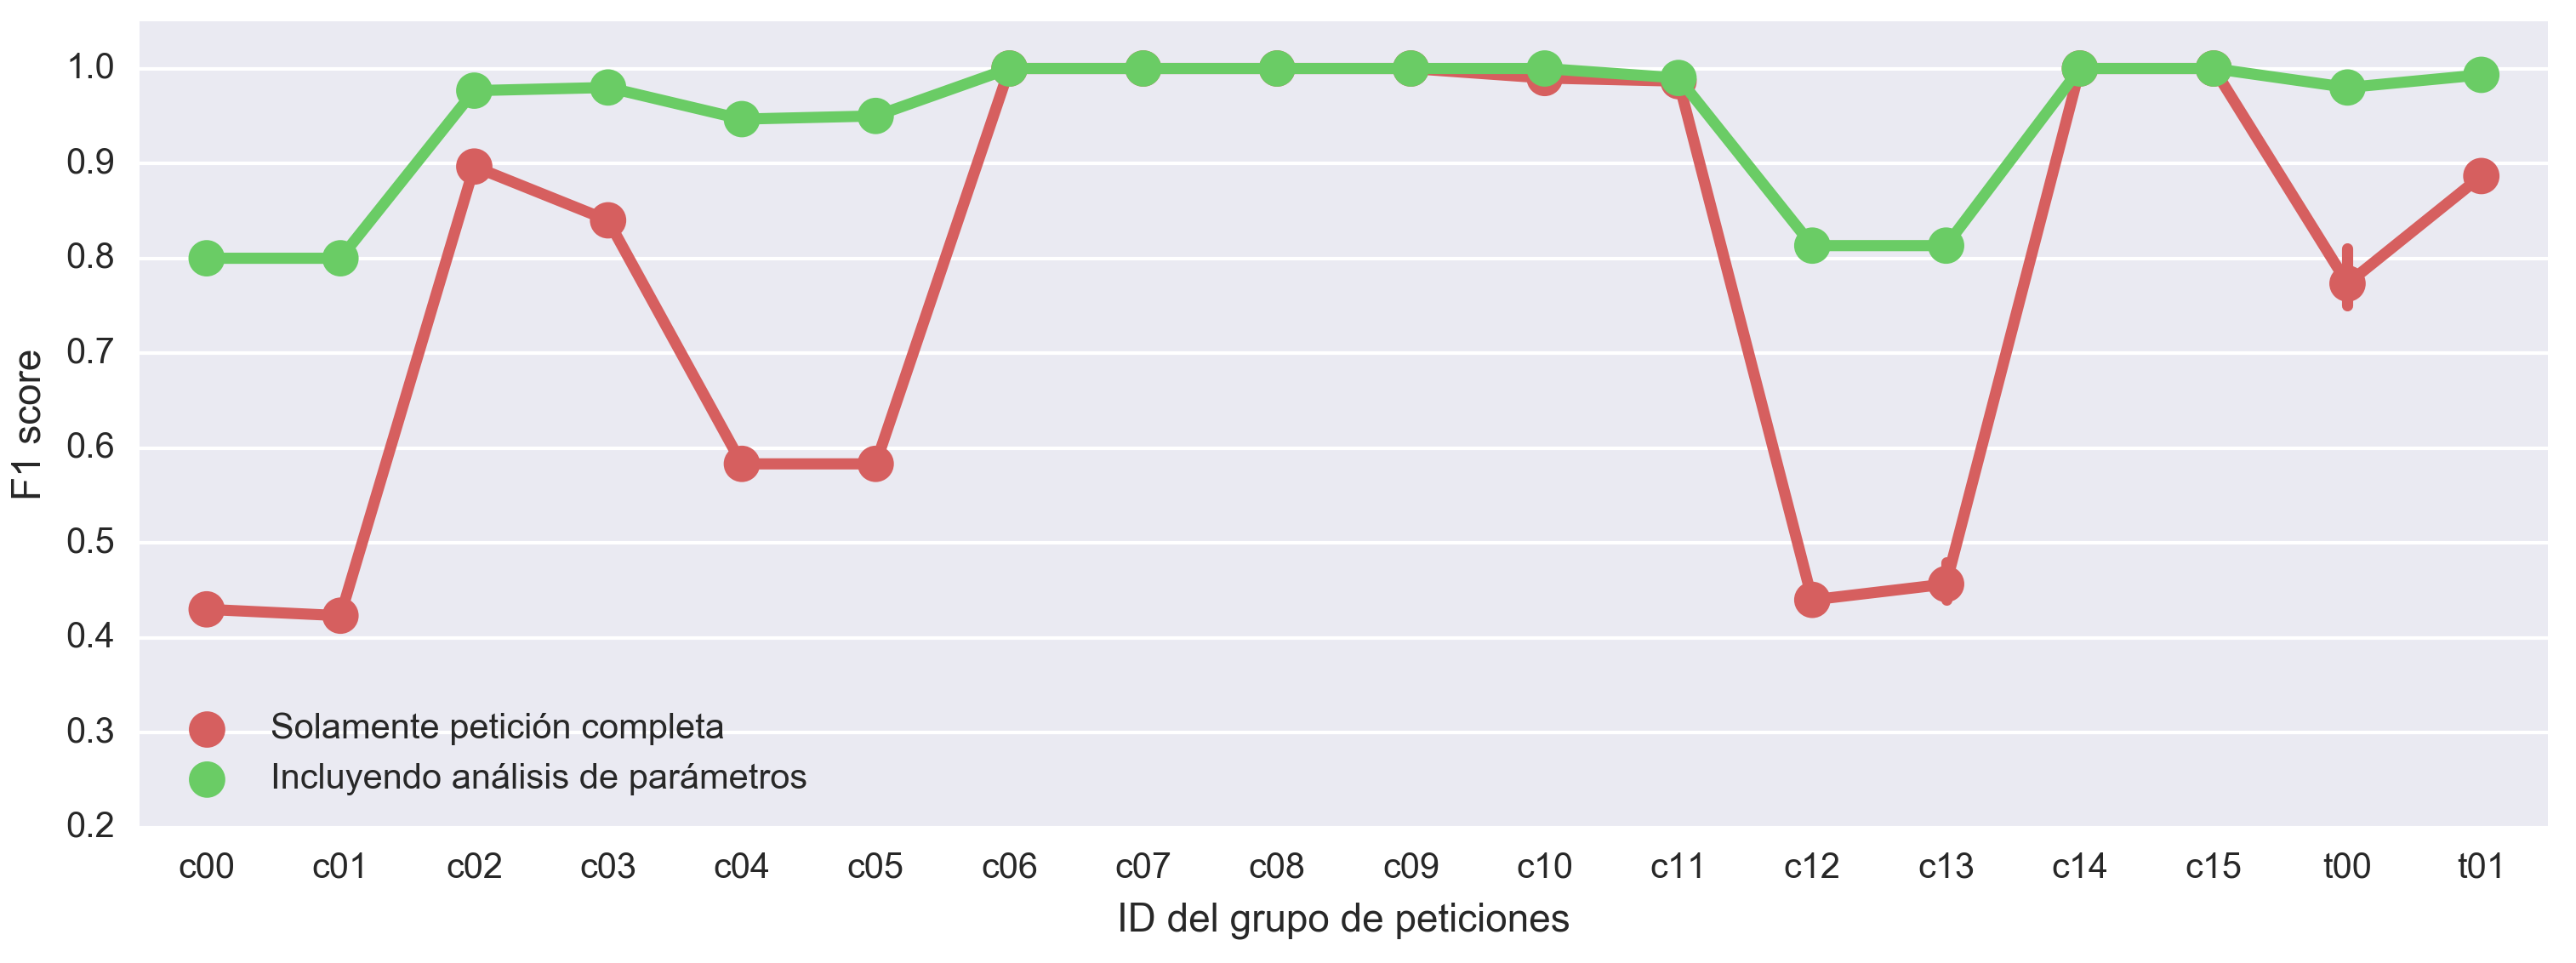
\includegraphics[width=\linewidth]{images/results-features.png}

    \caption{Resultados de detección que muestran las mejoras obtenidas
        con el análisis de valores de parámetros, incluyendo el escalamiento
        de \textit{features}.}
    \label{fig:res:results_features}
\end{figure}

En la \autoref{tbl:res:results_features} y también en la
\autoref{fig:res:results_features} se puede observar los resultados de
la clasificación usando solamente la petición completa, comparado con
los resultados obtenidos incluyendo el análisis de valores de parámetros.
Para ambos casos usamos 1500 peticiones para el entrenamiento de cada
grupo (cerca del 75\% de las muestras) e incluimos el escalamiento de
\textit{features}.
En los resultados promedios de todos los grupos (la última fila de la
tabla) se puede ver que con el análisis de parámetros el \gls{acr3:tpr}
mejora de \num{0.77} a \num{0.93}, el \gls{acr3:fpr} mejora de \num{0.11}
a \num{0.03} y el F$_{1}$-\textit{score} mejora de \num{0.79} a \num{0.95}.

\begin{table}[hbt]
    \centering
    \small
    \begin{tabularx}{\linewidth}{|c|CCC|CCC|}
        \hline
        ID  & \multicolumn{3}{c|}{Solamente petición completa}                                        & \multicolumn{3}{c|}{Incluyendo análisis de parámetros}                                  \\
            & \gls{acr3:tpr}              & \gls{acr3:fpr}              & F$_{1}$-\textit{score}      & \gls{acr3:tpr}              & \gls{acr3:fpr}              & F$_{1}$-\textit{score}      \\
        \specialrule{1.5pt}{0}{0}
        c00 & \num{0.32} $\pm$ \num{0.00} & \num{0.10} $\pm$ \num{0.01} & \num{0.43} $\pm$ \num{0.00} & \num{0.71} $\pm$ \num{0.01} & \num{0.05} $\pm$ \num{0.00} & \num{0.80} $\pm$ \num{0.00} \\ \hline
        c01 & \num{0.31} $\pm$ \num{0.01} & \num{0.10} $\pm$ \num{0.01} & \num{0.42} $\pm$ \num{0.01} & \num{0.72} $\pm$ \num{0.01} & \num{0.05} $\pm$ \num{0.01} & \num{0.80} $\pm$ \num{0.00} \\ \hline
        c02 & \num{0.89} $\pm$ \num{0.03} & \num{0.07} $\pm$ \num{0.05} & \num{0.90} $\pm$ \num{0.01} & \num{1.00} $\pm$ \num{0.00} & \num{0.03} $\pm$ \num{0.01} & \num{0.98} $\pm$ \num{0.01} \\ \hline
        c03 & \num{0.82} $\pm$ \num{0.01} & \num{0.10} $\pm$ \num{0.01} & \num{0.84} $\pm$ \num{0.00} & \num{1.00} $\pm$ \num{0.00} & \num{0.03} $\pm$ \num{0.00} & \num{0.98} $\pm$ \num{0.00} \\ \hline
        c04 & \num{0.83} $\pm$ \num{0.30} & \num{0.70} $\pm$ \num{0.52} & \num{0.58} $\pm$ \num{0.01} & \num{0.91} $\pm$ \num{0.01} & \num{0.01} $\pm$ \num{0.00} & \num{0.95} $\pm$ \num{0.01} \\ \hline
        c05 & \num{0.65} $\pm$ \num{0.30} & \num{0.40} $\pm$ \num{0.52} & \num{0.58} $\pm$ \num{0.01} & \num{0.92} $\pm$ \num{0.01} & \num{0.01} $\pm$ \num{0.00} & \num{0.95} $\pm$ \num{0.00} \\ \hline
        c06 & \num{0.99} $\pm$ \num{0.00} & \num{0.00} $\pm$ \num{0.00} & \num{1.00} $\pm$ \num{0.00} & \num{0.99} $\pm$ \num{0.00} & \num{0.00} $\pm$ \num{0.00} & \num{1.00} $\pm$ \num{0.00} \\ \hline
        c07 & \num{0.99} $\pm$ \num{0.00} & \num{0.00} $\pm$ \num{0.00} & \num{1.00} $\pm$ \num{0.00} & \num{0.99} $\pm$ \num{0.00} & \num{0.00} $\pm$ \num{0.00} & \num{1.00} $\pm$ \num{0.00} \\ \hline
        c08 & \num{1.00} $\pm$ \num{0.00} & \num{0.00} $\pm$ \num{0.00} & \num{1.00} $\pm$ \num{0.00} & \num{1.00} $\pm$ \num{0.00} & \num{0.00} $\pm$ \num{0.00} & \num{1.00} $\pm$ \num{0.00} \\ \hline
        c09 & \num{1.00} $\pm$ \num{0.00} & \num{0.00} $\pm$ \num{0.00} & \num{1.00} $\pm$ \num{0.00} & \num{1.00} $\pm$ \num{0.00} & \num{0.00} $\pm$ \num{0.00} & \num{1.00} $\pm$ \num{0.00} \\ \hline
        c10 & \num{0.99} $\pm$ \num{0.00} & \num{0.01} $\pm$ \num{0.01} & \num{0.99} $\pm$ \num{0.00} & \num{1.00} $\pm$ \num{0.00} & \num{0.00} $\pm$ \num{0.00} & \num{1.00} $\pm$ \num{0.00} \\ \hline
        c11 & \num{0.99} $\pm$ \num{0.01} & \num{0.01} $\pm$ \num{0.01} & \num{0.99} $\pm$ \num{0.01} & \num{1.00} $\pm$ \num{0.00} & \num{0.01} $\pm$ \num{0.00} & \num{0.99} $\pm$ \num{0.00} \\ \hline
        c12 & \num{0.33} $\pm$ \num{0.00} & \num{0.10} $\pm$ \num{0.01} & \num{0.44} $\pm$ \num{0.00} & \num{0.74} $\pm$ \num{0.00} & \num{0.05} $\pm$ \num{0.01} & \num{0.81} $\pm$ \num{0.01} \\ \hline
        c13 & \num{0.35} $\pm$ \num{0.04} & \num{0.13} $\pm$ \num{0.05} & \num{0.46} $\pm$ \num{0.02} & \num{0.74} $\pm$ \num{0.00} & \num{0.05} $\pm$ \num{0.01} & \num{0.81} $\pm$ \num{0.01} \\ \hline
        c14 & \num{1.00} $\pm$ \num{0.00} & \num{0.00} $\pm$ \num{0.00} & \num{1.00} $\pm$ \num{0.00} & \num{1.00} $\pm$ \num{0.00} & \num{0.00} $\pm$ \num{0.00} & \num{1.00} $\pm$ \num{0.00} \\ \hline
        c15 & \num{1.00} $\pm$ \num{0.00} & \num{0.00} $\pm$ \num{0.00} & \num{1.00} $\pm$ \num{0.00} & \num{1.00} $\pm$ \num{0.00} & \num{0.00} $\pm$ \num{0.00} & \num{1.00} $\pm$ \num{0.00} \\ \hline
        t00 & \num{0.67} $\pm$ \num{0.05} & \num{0.10} $\pm$ \num{0.08} & \num{0.77} $\pm$ \num{0.03} & \num{0.99} $\pm$ \num{0.01} & \num{0.06} $\pm$ \num{0.04} & \num{0.98} $\pm$ \num{0.00} \\ \hline
        t01 & \num{0.82} $\pm$ \num{0.01} & \num{0.10} $\pm$ \num{0.01} & \num{0.89} $\pm$ \num{0.01} & \num{1.00} $\pm$ \num{0.00} & \num{0.09} $\pm$ \num{0.06} & \num{0.99} $\pm$ \num{0.01} \\
        \specialrule{1.5pt}{0}{0}
            & \num{0.77} $\pm$ \num{0.28} & \num{0.11} $\pm$ \num{0.22} & \num{0.79} $\pm$ \num{0.23} & \num{0.93} $\pm$ \num{0.11} & \num{0.03} $\pm$ \num{0.03} & \num{0.95} $\pm$ \num{0.08} \\ \hline
    \end{tabularx}

    \caption{Resultados de detección que muestran las mejoras obtenidas
        con el análisis de valores de parámetros, incluyendo el escalamiento
        de \textit{features}.}
    \label{tbl:res:results_features}
\end{table}

De esta forma, los resultados obtenidos muestran la utilidad del análisis
de valores de los parámetros de las peticiones. A parte eso, se puede
notar una reducción de la varianza en las tres métricas, lo que indica
que se redujeron también las diferencias entre los resultados al utilizar
distintos subconjuntos de peticiones para el entrenamiento. Esto es un
indicador de robustez de \gls{acr3:name}, mostrando que con el análisis
de parámetros es menos susceptible a cambios por la elección de peticiones
de entrenamiento.


\subsection{Influencia de la cantidad de peticiones de entrenamiento}

Para que \gls{acr3:name} pueda realizar un buen trabajo de detección,
es necesario que los datos de entrenamiento cubran la mayor cantidad
posible de situaciones que se puedan dar posteriormente en la fase de
detección. Esto puede significar que se tenga que pasar una gran cantidad
de datos al \gls{acr3:waf} para realizar el entrenamiento. Pero el simple
hecho de aumentar la cantidad de peticiones para esta fase no siempre
es la mejor solución, ya que eso aumenta el tiempo que dura la fase de
entrenamiento y además no nos asegura que se cubran realmente todos los
casos normales posibles.

Los conjuntos de datos de prueba que utilizamos nos proveen con \num{2000}
peticiones normales en la mayoría de los grupos, como ya se mostró en la
\autoref{tbl:res:selected_data_sets}. Realizamos una prueba para analizar
los resultados que se obtienen al utilizar distintas cantidades de esos
datos normales para el entrenamiento, siempre incluyendo el escalamiento
de \textit{features} y el análisis de valores de parámetros.

\begin{table}[ht]
    \centering
    \small
    \begin{tabularx}{\linewidth}{|c|CCC|}
        \hline
        Cantidad de peticiones & \multicolumn{3}{c|}{Promedio de los 18 grupos}                                          \\
        de entrenamiento       & \gls{acr3:tpr}              & \gls{acr3:fpr}              & F$_{1}$-\textit{score}      \\
        \specialrule{1.5pt}{0}{0}
        \num{200}              & \num{0.92} $\pm$ \num{0.11} & \num{0.07} $\pm$ \num{0.06} & \num{0.92} $\pm$ \num{0.09} \\ \hline
        \num{500}              & \num{0.94} $\pm$ \num{0.09} & \num{0.06} $\pm$ \num{0.06} & \num{0.93} $\pm$ \num{0.09} \\ \hline
        \num{1000}             & \num{0.93} $\pm$ \num{0.11} & \num{0.03} $\pm$ \num{0.03} & \num{0.94} $\pm$ \num{0.08} \\ \hline
        \num{1500}             & \num{0.93} $\pm$ \num{0.11} & \num{0.03} $\pm$ \num{0.03} & \num{0.95} $\pm$ \num{0.08} \\ \hline
    \end{tabularx}

    \caption{Resultados de detección que muestran la influencia de la
        cantidad de peticiones de entrenamiento, incluyendo el escalamiento
        de \textit{features} y el análisis de valores de parámetros.}
    \label{tbl:res:results_training_samples}
\end{table}

Como se puede observar en la \autoref{tbl:res:results_training_samples},
utilizamos 200, 500, \num{1000} y \num{1500} peticiones para esta prueba,
que equivale a 10\%, 25\%, 50\% y 75\% de los datos disponibles en la
mayoría de los grupos. Los mejores resultados obtuvimos para la mayor
cantidad de peticiones utilizadas, aunque las diferencias comparado a las
demás cantidades son pequeñas y se podría usar también menos peticiones
sin una degradación significativa de la eficacia de detección.
Por esta razón también utilizamos 1500 peticiones para el entrenamiento
en las pruebas presentadas en las secciones anteriores.


\subsection{Influencia de anomalías en los datos de entrenamiento}

Un desafío en ambientes reales es asegurar que los datos de entrenamiento
solamente contengan peticiones \gls{acr3:http} normales y que no haya
ninguna anomalía entre ellas. La presencia de ruido (es decir, anomalías)
en los datos de entrenamiento puede reducir la capacidad de clasificación
del \gls{acr3:ocsvm}, ya que esas anomalías influyen en la posición de
la superficie separadora y consecuentemente esto llevará a resultados
diferentes en la posterior fase de detección.
Como ya presentamos en el capítulo \autoref{chap:p3_concepts_ocsvm}, el
clasificador en cuestión tiene la capacidad de dejar ciertas muestras al
mismo lado del hiperplano que el origen durante la fase de entrenamiento,
de manera que cuenta con cierta capacidad para reducir la influencia de
peticiones anómalas (que son muestras positivas o ataques) que se encuentren
dentro de los datos de entrenamiento. En esta prueba buscamos descubrir
cómo esto se refleja en el desempeño de detección de \gls{acr3:name}.

Realizamos una prueba para analizar en qué manera el \gls{acr3:ocsvm}
se ve afectado en su capacidad de clasificación con la presencia de
peticiones anómalas en los datos de entrenamiento. Para eso, incluimos
una cierta cantidad de anomalías dentro de las peticiones de entrenamiento
para llegar a 1\%, 5\% y 10\% de anomalías. Acá volvimos a utilizar 200,
500, \num{1000} y \num{1500} peticiones para el entrenamiento, siempre
incluyendo el escalamiento de \textit{features} y el análisis de valores
de parámetros.

\begin{figure}[ht]
    \centering
    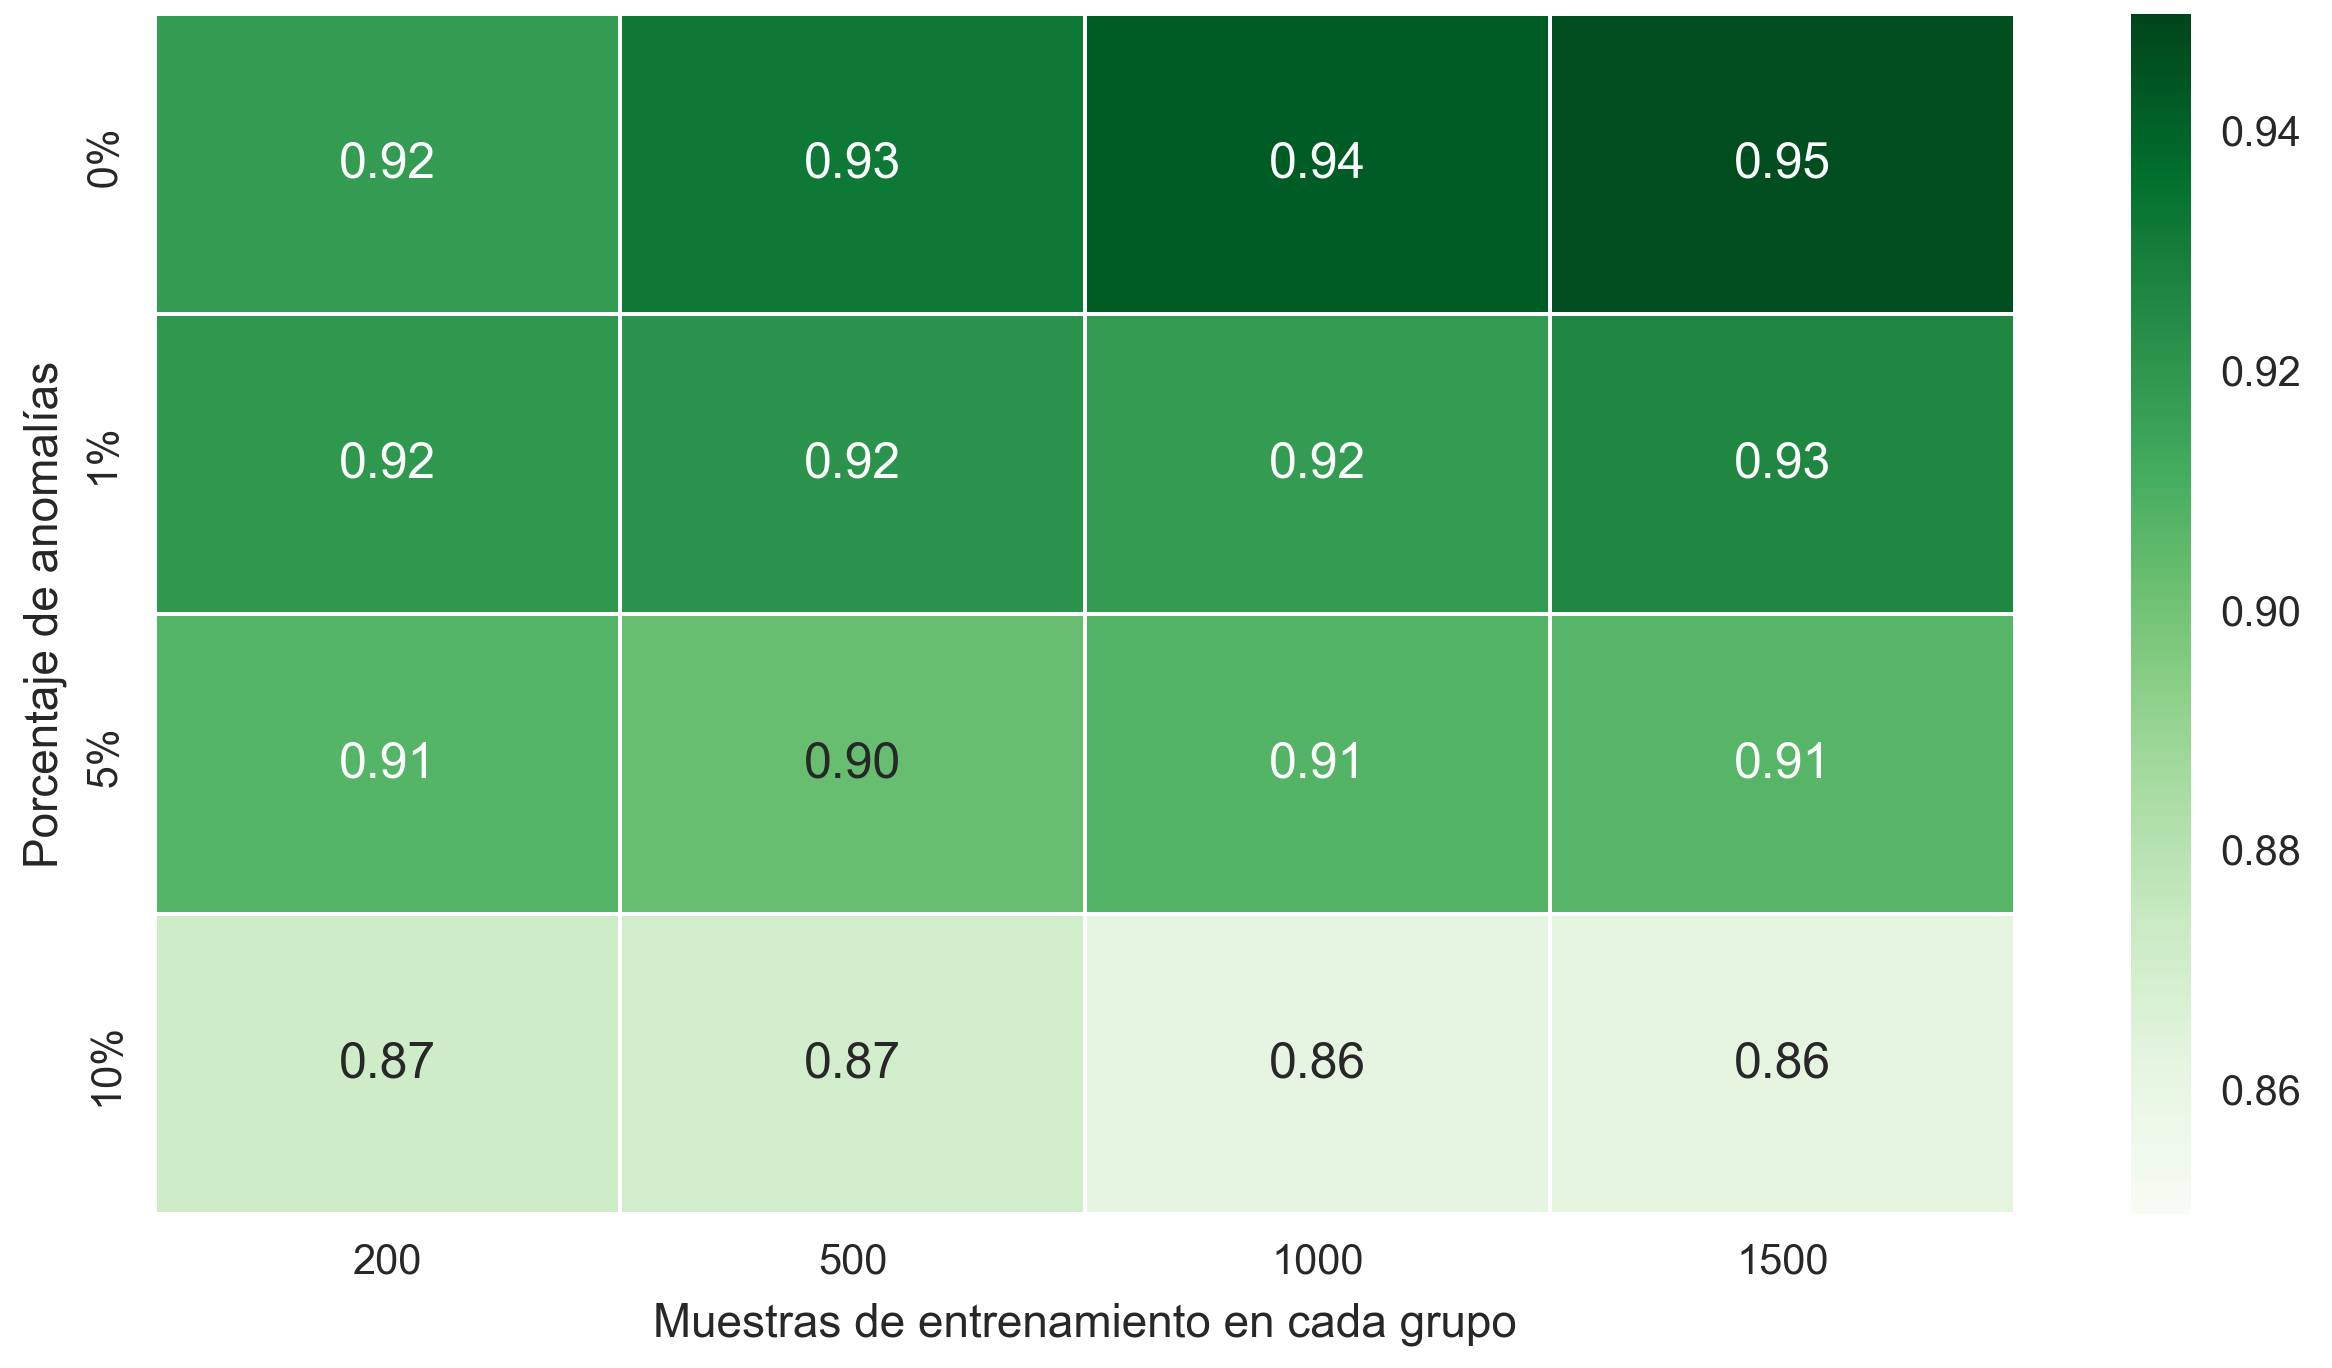
\includegraphics[width=\linewidth]{images/results-training-anomalies.png}

    \caption{Mapa de calor de los resultados de detección, en términos
        del F$_{1}$-\textit{score}, que muestran la influencia de la
        cantidad de peticiones y el porcentaje de anomalías en el
        entrenamiento, incluyendo el escalamiento de \textit{features}
        y el análisis de valores de parámetros.}
    \label{fig:res:results_training_anomalies}
\end{figure}

La \autoref{fig:res:results_training_anomalies} muestra un mapa de calor
(\textit{heatmap}) de los resultados de detección de esta prueba. Las
columnas contienen las distintas cantidad de peticiones utilizadas para
el entrenamiento, las filas representan diferentes porcentajes de anomalías
que se incluyeron en los datos de entrenamiento y los valores en cada celda
indican el F$_{1}$-\textit{score} promedio de los 18 grupos que se obtuvo
con esa configuración. Las celdas con colores más oscuros contienen
números mayores, lo que indica resultados mejores.

Como se puede ver en nuestros resultados, el F$_{1}$-\textit{score} sufre
una degradación gradual conforme va aumentando el porcentaje de anomalías,
aunque es una reducción poco significativa para 1\% de anomalías.
Esta degradación de la detección se da de forma similar para todas las
cantidad de peticiones utilizadas para el entrenamiento, aunque el caso
más pronunciado se da para la mayor cantidad de peticiones. Esto se debe
a que ya se tiene mayor cantidad de anomalías presentes, por ejemplo
con 10\% de \num{1500} peticiones ya hay 150 muestras anómalas que ejercen
influencia sobre la posición y forma de la superficie separadora de los
clasificadores, lo que se ve reflejado en los resultados.

Cabe resaltar que un 10\% de anomalías de entrenamiento ya es un porcentaje
muy elevado de ruido. En ese caso se debería utilizar alguna estrategia
adicional para obtener un conjunto de datos de entrenamiento más limpio,
como por ejemplo una clasificación previa con aprendizaje no supervisado,
con el fin de reducir el impacto negativo sobre la eficacia de detección
del \gls{acr3:waf}.

De esta forma, los resultados obtenidos en esta prueba muestran que
\gls{acr3:name} con sus clasificadores \gls{acr3:ocsvm} presenta cierta
robustez frente a la presencia de algunas pocas anomalías en los datos
de entrenamiento.


\section{Análisis del tiempo de respuesta de las aplicaciones protegidas}

Esta prueba que realizamos con \gls{acr3:name} apunta a cuantificar en
qué medida se ve afectado el tiempo de respuesta de las aplicaciones web
que nuestra implementación debe proteger.
Si este tiempo de respuesta aumenta de gran manera debido al uso del
\gls{acr3:waf}, las aplicaciones podrían quedar inutilizables para el
usuario final, significando que nuestra implementación no puede ser
usada para detección en tiempo real.
Estamos conscientes de que las mediciones realizadas durante esta prueba
no necesariamente reflejan un ambiente real, pero sí nos permiten establecer
el orden de magnitud de la variación que introduce \gls{acr3:name} en
el tiempo de respuesta de las aplicaciones protegidas.

Para esta prueba, nosotros creamos una simple aplicación capaz de recibir
peticiones \gls{acr3:http} y enviar las respuestas correspondientes, con
el fin de simular aplicaciones web protegidas por \gls{acr3:name}.
Posteriormente medimos el intervalo de tiempo entre el envío de una petición
a esa aplicación y la recepción de la respuesta.
Realizamos esta medición con tres configuraciones distintas. En la primera
configuración se enviaron las peticiones directamente a la aplicación
destino sin pasar por \gls{acr3:name}, para obtener así el tiempo de
respuesta normal. En la segunda configuración el tráfico fue enviado a
través del \gls{acr3:waf} pero sin que este realice las tareas de detección,
para de esta manera medir el retraso incurrido por agregar un componente
al camino de los paquetes. En la última configuración las peticiones
pasaron por un \gls{acr3:waf} previamente entrenado, con el fin de medir
el retraso ocasionado al utilizar las funciones de detección.

El código de todas las partes utilizadas en esta prueba esta en nuestro
repositorio público, en el directorio \path{/tests/waf_speed/}. Ejecutamos
todos los procesos en una misma máquina, buscando reducir de esta manera
diferentes variables presentes en la red y concentrarnos en el retraso
introducido por el uso del \gls{acr3:waf}.
La máquina utilizada tiene una plataforma \textit{Ubuntu 14.04} de 64
\textit{bits}, con un procesador \textit{Intel i5} de \num{1.7} \gls{acr3:ghz}
y 8 \gls{acr3:gb} de memoria \gls{acr3:ram}.

\begin{table}[ht]
    \centering
    \small
    \begin{tabularx}{\linewidth}{|l|C|}
        \hline
        \multicolumn{1}{|c|}{Configuración}   & Tiempo de respuesta promedio (milisegundos) \\
        \specialrule{1.5pt}{0}{0}
        Sin \gls{acr3:waf}                    &  \num{4.8} $\pm$ \num{2.2} \\ \hline
        Con \gls{acr3:waf} pero sin detección &  \num{6.4} $\pm$ \num{1.7} \\ \hline
        Con \gls{acr3:waf} y con detección    & \num{10.1} $\pm$ \num{2.6} \\ \hline
    \end{tabularx}

    \caption{Resultados de la prueba de tiempo de respuesta de las
        aplicaciones protegidas.}
    \label{tbl:res:test_2}
\end{table}

En la \autoref{tbl:res:test_2} se pueden ver los resultados de esta
prueba. Para cada una de las tres configuraciones cronometramos 160
peticiones pertenecientes a distintos grupos de método y \gls{acr3:url},
de las cuales la mitad fueron peticiones normales y la otra mitad anomalías.
No pudimos percibir diferencias significativas de tiempo entre peticiones
normales y anómalas, ni tampoco entre peticiones de distintos grupos
(con distintas cantidades de parámetros). Posibles variaciones están
contenidas dentro de la desviación estándar indicada en la tabla mencionada.
Los resultados se mantuvieron constantes en repeticiones de la misma prueba.

La configuración sin \gls{acr3:name} obtuvo el menor tiempo de respuesta,
con un promedio de \num{4.8} milisegundos.
En la segunda configuración, que utiliza \gls{acr3:name} sin detección,
se obtuvo un retardo adicional de \num{1.6} milisegundos en tiempo de
respuesta comparado al primer caso. La tercera configuración, que incluye
la detección, obtuvo retardos adicionales de \num{5.3} y \num{3.7}
milisegundos comparado con las dos primeras configuraciones respectivamente.
Esto indica el orden de magnitud del retraso que \gls{acr3:name} podría
agregar a las peticiones. Se espera que esto sea un límite superior
para un \gls{acr3:waf} optimizado (incluso utilizando otro lenguaje).

Además, considerando que la latencia promedio de paquetes de red en
Internet está entre 200 y 300 milisegundos \citep{internetWeatherMap}
y será un poco mayor a eso para mensajes \gls{acr3:http}, se espera que
estos pocos milisegundos adicionales agregados por \gls{acr3:name} no
afectarán de forma notable el tiempo de respuesta de las aplicaciones
web protegidas.
Para aplicaciones dentro de una red interna de alta velocidad, el retraso
podría llegar a ser perceptible, pero nuestra implementación fue hecha
en primer lugar para aplicaciones accesibles a través de Internet, como
fue explicado en la introducción en el \autoref{chap:p3_introduction}.


\section{Análisis del tiempo de entrenamiento}

En esta última prueba realizada se analizó la relación que existe entre
el tiempo de entrenamiento de \gls{acr3:name} (que incluye el tiempo
consumido por los procesos de extracción de \textit{features} y los
clasificadores \gls{acr3:ocsvm} empleados) y la cantidad de peticiones
\gls{acr3:http} utilizadas para dicho entrenamiento.

La duración estimada del entrenamiento es una información importante
para los administradores responsables por \gls{acr3:name}, ya que estas
personas necesitan saber si el entrenamiento durará minutos, horas o días,
a fin de poder planificar los momentos adecuados para este proceso.
De la misma manera que en la prueba anterior, estamos conscientes de que
las mediciones realizadas durante esta prueba no necesariamente reflejan
un ambiente real con un \gls{acr3:waf} optimizado (incluso utilizando otro
lenguaje de programación), pero sí nos permiten establecer el orden de
magnitud del tiempo de entrenamiento de nuestra implementación y la relación
entre este tiempo y la cantidad de peticiones que fueron utilizadas.

El código para esta prueba también esta en nuestro repositorio público,
en el directorio \path{/tests/training_duration/}.
Volvimos a utilizar la misma máquina para ejecutar las pruebas, que tiene
una plataforma \textit{Ubuntu 14.04} de 64 \textit{bits}, con un procesador
\textit{Intel i5} de \num{1.7} \gls{acr3:ghz} y 8 \gls{acr3:gb} de memoria
\gls{acr3:ram}.

\begin{table}[ht]
    \centering
    \small
    \begin{tabularx}{\linewidth}{|r|C|C|r|}
        \hline
        \multicolumn{1}{|c|}{\begin{tabular}[c]{@{}c@{}}Cantidad de\\ peticiones\end{tabular}}
        & \multicolumn{1}{c|}{\begin{tabular}[c]{@{}c@{}}Tiempo promedio\\ por petición (segundos)\end{tabular}}
        & \multicolumn{1}{c|}{\begin{tabular}[c]{@{}c@{}}Tiempo máximo\\ por petición (segundos)\end{tabular}}
        & \multicolumn{1}{c|}{\begin{tabular}[c]{@{}c@{}}Tiempo total\\ máximo (segundos)\end{tabular}} \\
        \specialrule{1.5pt}{0}{0}
        \num{10}     & \num{0.0013} $\pm$ \num{0.0004} & \num{0.0020} &   \num{0.0195} \\ \hline
        \num{100}    & \num{0.0011} $\pm$ \num{0.0004} & \num{0.0017} &   \num{0.1724} \\ \hline
        \num{1000}   & \num{0.0010} $\pm$ \num{0.0004} & \num{0.0017} &   \num{1.7126} \\ \hline
        \num{10000}  & \num{0.0011} $\pm$ \num{0.0004} & \num{0.0018} &  \num{17.9132} \\ \hline
        \num{100000} & \num{0.0020} $\pm$ \num{0.0005} & \num{0.0070} & \num{703.9531} \\ \hline
    \end{tabularx}

    \caption{Resultados de la prueba de tiempo de entrenamiento.}
    \label{tbl:res:test_3}
\end{table}

La \autoref{tbl:res:test_3} muestra los resultados de esta prueba, indicando
el tiempo por petición que se alcanzó para las diferentes cantidades
utilizadas para el entrenamiento. Para cada una de estas cantidades,
realizamos entrenamientos con cada uno los grupos de \gls{acr3:url} y
método \gls{acr3:http}.
Cabe mencionar que el tiempo de entrenamiento de cada clasificador está
influenciado por la cantidad de \textit{features} extraídos en cada uno
de estos grupos de peticiones y debido a esto el tiempo medido puede ser
diferente para cada grupo. La tabla de resultados muestra el tiempo
promedio y también el tiempo máximo; este último puede ser utilizada a
modo de establecer un límite superior de la duración del entrenamiento.

En la tabla mencionada podemos observar que el tiempo de entrenamiento
máximo está en el orden de algunos milisegundos por petición, específicamente
el máximo está en 7 milisegundos. Esto significa que el entrenamiento
de \gls{acr3:name} puede tardar unos 704 segundos (cerca de 12 minutos)
para una cantidad de \num{100000} peticiones.
En nuestra opinión, este tiempo es muy manejable, permitiendo que el
\gls{acr3:waf} pueda ser entrenado con nuevos datos en cuestión de
minutos en los momentos que el administrador del mismo lo considere
necesario.


\section{Comparación con trabajos relacionados}

En esta sección queremos comparar nuestro implementación y los resultados
que obtuvimos con algunos trabajos de autores relacionados al área de
\gls{acr3:ids} con detección de anomalías. Nos enfocamos en trabajos que
utilizan los mismos conjuntos de datos que nosotros empleamos. En la
\autoref{tbl:res:comparison} se muestra un resumen de la comparación de
resultados de nuestra implementación con trabajos de otros investigadores.

\begin{table}[ht]
    \centering
    \small
    \begin{tabularx}{\linewidth}{|l|X|c|c|c|}
        \hline
        \multicolumn{1}{|c|}{Sistema de detección} & \multicolumn{1}{c|}{Observaciones}         & \gls{acr3:tpr} & \gls{acr3:fpr} & F$_{1}$-\textit{score} \\
        \specialrule{1.5pt}{0}{0}
        \gls{acr3:name}                            & \gls{acr3:ocsvm}s con cantidad variable de & \num{0.93}     & \num{0.03}     & \num{0.95}             \\
        (el presente trabajo)                      & \textit{features}                          &                &                &                        \\ \hline
        \textit{ModSecurity}                       & popular detector por firmas de ataques     & \num{0.56}     & \num{0.00}     & \num{0.71}             \\
        \citep{gimenez2015tfg}                     &                                            &                &                &                        \\ \hline
        \textit{HTTP-WS-AD}                        & modelos estadísticos con agregación y      & \num{0.99}     & \num{0.02}     & \num{0.99}             \\
        \citep{gimenez2015tfg}                     & cascada                                    &                &                &                        \\ \hline
        \citep{torranoGimenez2015study}            & promedio de cuatro tipos distintos de      & \num{0.95}     & \num{0.05}     & -                      \\
                                                   & árboles de decisión                        &                &                &                        \\ \hline
        \textit{OC-WAD}                            & conjunto de \gls{acr3:ocsvm}s con          & \num{0.96}     & \num{0.03}     & -                      \\
        \citep{parhizkar2015oc}                    & cantidad fija de \textit{features}         &                &                &                        \\ \hline
    \end{tabularx}

    \caption{Comparación de resultados de \gls{acr3:name} con otros trabajos
        que utilizan también el conjunto de datos \gls{acr3:csic} 2010.}
    \label{tbl:res:comparison}
\end{table}

Antes de analizar otras propuestas de detección de anomalías, investigamos
sobre \gls{acr3:ids} basados en firmas de ataques (no realizan detección
de anomalías) para tener una referencia sobre este tipo de sistemas de
detección. Una implementación popular de un \gls{acr3:waf} basados en
firmas es \textit{ModSecurity}.
En \citep{gimenez2015tfg} % from section 5.3.2 - tabla 5.25 CSIC-ModSecurity
el autor aplicó este detector al conjunto de datos \gls{acr3:csic} 2010,
utilizando las firmas de ataques que el mismo trae por defecto. Así obtuvo
un \gls{acr3:tpr} de \num{0.56}, un \gls{acr3:fpr} de \num{0.00} y un
F$_{1}$-\textit{score} de \num{0.71}. Una fortaleza de este detector es que
no incurre en falsos positivos (peticiones normales detectadas como ataques).
Pero nuestra implementación obtiene una detección significativamente mejor
que este popular detector basado en firmas de ataques, como se puede ver
en los resultados de la ya mencionada \autoref{tbl:res:comparison}.

En \citep{gimenez2015tfg} % from section 6.1.6 - conclusiones
se presenta un detector de anomalías llamado \textit{HTTP-WS-AD}.
En este trabajo se utilizan varios modelos estadísticos y se realizan
pruebas con varios esquemas de agregación y cascada de modelos para
mejorar los resultados de la detección de peticiones \gls{acr3:http}
anómalas. El autor reporta haber obtenido un \gls{acr3:tpr} de \num{0.99},
un \gls{acr3:fpr} de \num{0.02} y un F$_{1}$-\textit{score} de \num{0.99}
para el conjunto de datos \gls{acr3:csic} 2010.
Cada una de estos tres resultados es levemente superior a los números
logrados por \gls{acr3:name}, con la notable diferencia de que este
trabajo utiliza métodos estadísticos mientras que nuestra implementación
emplea herramientas del área de \gls{acr3:ml}.
Además, Giménez también realizó mediciones del impacto de su detector
en el tiempo de respuesta de las aplicaciones web protegidas, reportando
un retraso adicional promedio de 50 milisegundos introducido por las tareas
de detección. % from table 5.27 - CSIC-Medición de Tiempos de Respuesta
\gls{acr3:name} obtuvo un retraso promedio menor a 10 milisegundos en
nuestras pruebas, mostrando una leve ventaja en este aspecto frente a
\textit{HTTP-WS-AD}.

En la segunda parte del trabajo
\citep{torranoGimenez2015study} % from section 6.2 - second point in conclusions
se presenta un detector de anomalías que utiliza cuatro tipos de árboles
de decisiones para su proceso de detección. Estos árboles son también
herramientas de clasificación del área de \gls{acr3:ml}, pero en este
caso se trata de clasificadores binarios o de dos clases. Esto significa
que se entrena los clasificadores con peticiones normales y anómalas.
El trabajo en cuestión reporta haber obtenido un \gls{acr3:tpr} de \num{0.95}
y un \gls{acr3:fpr} de \num{0.05} sobre el conjunto de datos \gls{acr3:csic}
2010. \gls{acr3:name} obtuvo un \gls{acr3:tpr} inferior con \num{0.93},
pero obtuvo un \gls{acr3:fpr} superior de \num{0.03}.
Cabe resaltar que el trabajo en cuestión entrena sus clasificadores con
ambas clases de peticiones (normales y anomalías), mientras que nosotros
entrenamos con peticiones normales únicamente. Creemos que debido a eso,
\gls{acr3:name} es más robusto frente a la aparición de nuevos tipos de
ataques, ya que no se usan anomalías en el entrenamiento.

En \citep{parhizkar2015oc} % from section VI - conclusions
se presenta un detector de anomalías llamado \textit{OC-WAD} para peticiones
\gls{acr3:http}. Los autores extraen una cantidad fija de \textit{features}
de las peticiones y posteriormente utilizan un conjunto de clasificadores
\gls{acr3:ocsvm} con \textit{kernel} \gls{acr3:rbf} para realizar la
detección. Los distintos clasificadores son entrenados con diferentes
subconjuntos de \textit{features}. Además, ellos presentan un algoritmo
de enjambres llamado \textit{BeeSnips}, que utilizan para la creación
y optimización del conjunto de clasificadores.
Trabajando con el conjunto de datos \gls{acr3:csic} 2010, los autores
reportan haber obtenido un \gls{acr3:tpr} de \num{0.96} y un \gls{acr3:fpr}
de \num{0.03}. Estos resultados son similares a los nuestros; obtuvimos
un \gls{acr3:tpr} inferior de \num{0.93} y un \gls{acr3:fpr} igual de
\num{0.03}. Pero en este trabajo nos se brinda mucha información sobre
la manera que realizaron sus pruebas; por ejemplo no explican si entrenan
conjuntos de clasificadores separados por \gls{acr3:url}, lo que nos
deja dudas sobre cuan comparables son nuestros resultados.
